\documentclass[reprint,pre,amsmath,amssymb,superscriptaddress,nofootinbib]{revtex4-2}
\usepackage{graphicx}
\usepackage{xcolor}
\definecolor{darkblue}{rgb}{0.1,0.2,0.5}
\usepackage{booktabs}
\usepackage[T1]{fontenc}
\usepackage{lmodern}
\usepackage[utf8]{inputenc}
\usepackage[colorlinks=true,linkcolor=darkblue,citecolor=darkblue,urlcolor=darkblue]{hyperref}
\graphicspath{{figs/}}
\newcommand{\sz}{s_0}
\newcommand{\szc}{s_0^{*}}

\begin{document}

\title{Threshold, nucleation and disorder pinning\\ in a chiral three-dimensional network of phase links\\ with a conserved budget}

\author{Vasyl Batrukh}
\email{batrukh@gmail.com}
\affiliation{Independent researcher}

\date{\today}

\begin{abstract}
We study a deterministic lattice dynamical system in three dimensions: complex amplitudes on the links of a tetrahedral network with a conserved total intensity (the budget), a real order parameter $\psi$ on the nodes, a frozen orientation field of the links and a weak chiral, non-reciprocal rotation of the link force. The system was built as a toy model of a pre-geometric medium; we keep its names (the Matrix, worlds, the arrow of time) as labels. Without rotation the homogeneous Matrix is stable and nothing forms, although at $s_0=3.0$ a planted nucleus larger than $R_c\approx2.4$ lattice spacings grows into a world; with rotation $\alpha=0.05$--0.2 a world---a region of the second phase of $\psi$---nucleates and grows in nearly every run (32 of 32 seeds on the plateau). Linearizing the coupled dynamics of intensity and $\psi$ gives a threshold of the budget, $s_0^*=2.864$ ($h=0.36$), that the full Jacobian reproduces to 0.005 after an extrapolation in box size that assumes $1/L^2$; the base point of the model lies just above it, where worlds must nucleate. The phases of four-link loops obey an Adler equation; the rotation unlocks them collectively, with no single-loop step, and a world expels the twist into the surrounding Matrix. At $\alpha=0.25$, $h=0.36$ and $L=16$, 7 of 24 arrow fields produce a stable finite island inside a living Matrix, and the place of the island is fixed by the arrows: with new noise it forms at the same place in 32 of 32 runs. Worlds also form, in 8 of 8 runs, on lattices grown from a phase-field crystal with their natural defects. Finally, near the threshold the Matrix responds to a local source as a soft medium near a linear instability: the halo is the exact linear response of the lattice, reproduced in shape to 1\,\% with no free parameters, with a range that grows as $s_0\to s_0^*$. We list ten negative results, and we state which ingredients are put in by hand.
\end{abstract}

\maketitle

%=====================================================================
\section{Introduction}\label{sec:intro}


In Part~I~\cite{Batrukh2026v1} we studied a two-dimensional toy model of a pre-geometric medium. There is no space with given laws, only a network of links, the \emph{Matrix}. Each link carries a complex amplitude, each node a real order parameter $\psi$, and the total intensity of the links---the \emph{budget}---is conserved. The two-dimensional network boils by itself, because the interaction between links is non-reciprocal, and in the boiling it nucleates finite \emph{worlds}: regions of the second phase of $\psi$ with a physical boundary. Inside worlds live a massless gauge mode, domains and Alice strings~\cite{Batrukh2026v1,Batrukh2026alice}.

Two dimensions, however, run into three walls, and none of them is technical. \emph{Gravity}: in two space dimensions general relativity has no local dynamics; a mass only cuts a cone out of space~\cite{Deser1984}. We saw exactly this---a lens without attraction---and an attractive $1/r$ force is impossible there by construction. \emph{Matter}: in two dimensions a topological defect is a point, and our vortices survived only in deep worlds, while the worlds of the base model are shallow. In three dimensions defects are lines, loops and monopoles, with a different topology and different chances to be stable. \emph{Dimension}: the question ``why three?'' cannot even be asked in a plane.

The move to three dimensions was not a mere change of lattice. With the parameters of Part~I transferred to a tetrahedral network, no world forms anywhere in the budget range $\sz=2.5$--$4.25$ (0 of 12 runs). Part~I even reported that in 3D coherent islands do not grow to critical size~\cite{Batrukh2026v1}. A world appears only with a weak chiral rotation of the link force and only in a narrow window of the budget. This raises the question of the present paper: what sets that window, and where in the network a world is born.

We answer it with three results.
(i) The threshold of the budget is \emph{derived}, not scanned: linearizing the coupled dynamics of link intensity and $\psi$ gives a determinant that vanishes at $\szc=2.864$, and the numerics agree (Sec.~\ref{sec:threshold}).
(ii) The place of birth is set by the arrow of time---the orientation field of the links---and not by chance: with the same arrows and new noise, the island forms at the same place in 32 of 32 runs (Sec.~\ref{sec:tau}).
(iii) Near the threshold the Matrix is soft: the halo around a local source is the linear response of the lattice, reproduced in shape to 1\,\% without free parameters, and its range grows as $\sz\to\szc$ (Sec.~\ref{sec:critical}).
Along the way we show that worlds also form on lattices grown from a field, with defects, and we list the negative results with their diagnosis (Sec.~\ref{sec:neg}).

\emph{What we do not claim.} The model is classical. It is not a theory of our universe. The lattice, the arrows and the chiral rotation are put in by hand; worlds, islands and the threshold emerge. Every number is given with the number of independent runs behind it.

%=====================================================================
\section{The model in three dimensions}\label{sec:model}

\emph{Network.} The nodes form a cubic lattice $L^3$ with periodic boundaries. Each node is joined to 14 neighbours: the six along the axes, six along face diagonals and two along a body diagonal (the Kuhn triangulation). Every cube is cut into six tetrahedra, so all cells of the network are tetrahedra. The lattice is put in by hand; in Sec.~\ref{sec:lattices} we replace it by lattices grown from a field.

\emph{Variables.} A link $e=(a\to b)$ carries a complex amplitude $z_e$; its intensity is $\rho_e=|z_e|^2$. A node carries a real order parameter $\psi_i$: the Matrix sits at $\psi_M<0$ ($\psi_M=-0.69$ at $h=0.36$), a world at $\psi>0$. The total intensity $S=\sum_e\rho_e$ is conserved exactly; the \emph{budget} is $\sz=S/m$, with $m=7L^3$ the number of links. Each tetrahedron contains three closed four-link loops $q$ with holonomy $P_q=z_1z_2z_3z_4$ (orientations included). The dynamics is invariant under $z_{ab}\to e^{i(\phi_a-\phi_b)}z_{ab}$ to machine precision ($10^{-14}$), so only $|z_e|$ and the loop holonomies are physical.

\emph{Arrows.} A frozen smooth random field $\tau_i$ (correlation length $\ell_\tau=4$) orients each link from smaller to larger $\tau$. The orientation fixes the sense in which the chiral rotation below acts on the link.

\emph{Equations of motion.} Time is first order (RK4, $dt=0.005$). With $\bar\psi_e=(\psi_a+\psi_b)/2$, $\Delta\psi_e=\psi_b-\psi_a$ and $w=\beta+\sqrt{\beta^2-1}$ the vacuum amplitude of a link,
\begin{align}
\dot z_e ={}& \Big[-1-|z_e|^2+\frac{\lambda_c\bar\psi_e}{2w^2}\Big]z_e-z_e\Pi_e \nonumber\\
&+(1+i\alpha)\Big[\beta_e F^{\beta}_e+F^{\varepsilon}_e-\frac{\kappa}{2w}(\Delta\psi_e)^2\frac{z_e}{|z_e|}\Big], \label{eq:z}\\
\dot\psi_i ={}& \psi_i-\psi_i^3+h+\kappa\sum_{e\ni i}\frac{|z_e|}{w}(\psi_j-\psi_i) \nonumber\\
&+\frac{\lambda_c}{4w^2}\sum_{e\ni i}\big(|z_e|^2-\sz\big)-\chi'(\psi_i)\sum_{q\ni i}\varepsilon_q c_q. \label{eq:psi}
\end{align}
In Eq.~(\ref{eq:psi}) $j$ is the other end of the link $e$; the sign convention of $\Delta\psi_e$ does not matter in Eq.~(\ref{eq:z}), where it enters squared.
Here $F^\beta_e=\partial_{\bar z_e}\sum_{q\ni e}\mathrm{Re}P_q|P_q|^{a-1}$ pulls loops towards flatness and amplitudes towards $w$; $a=3/4$ keeps the vacuum of a four-link loop equal to that of the triangle in Part~I, and $\beta_e=2\beta/(a k_e)$ with $k_e$ the number of loops through $e$. The term $F^\varepsilon_e$ is the cost of non-flat loops inside worlds, $\varepsilon_q c_q$ with $c_q=(|P_q|^a-\mathrm{Re}P_q|P_q|^{a-1})/4\ge 0$ and weight $\varepsilon_q=\varepsilon_0\langle\chi\rangle_q$, $\chi(\psi)=((1+\psi)/2)^2$. The last term of Eq.~(\ref{eq:z}) enforces conservation: the local change of intensity $s_e=2\mathrm{Re}(\bar z_e\dot z^{(0)}_e)$, with $\dot z^{(0)}_e$ the right-hand side of Eq.~(\ref{eq:z}) without the term $-z_e\Pi_e$, is spread over a neighbourhood by the kernel $K=P^n$ ($P$ the local averaging operator, $n=100$, range $\approx 10$ links) and removed,
\begin{equation}
\Pi_e=\frac{(Ks)_e+(\sum_f\rho_f-S)/m}{2\rho_e},
\end{equation}
so that $S$ is constant and the budget is redistributed with a delay.

\emph{What is put in by hand.} The lattice, the arrows $\tau$ and the chiral rotation $\alpha$ are postulates. So are the potentials in Eqs.~(\ref{eq:z})--(\ref{eq:psi}). Worlds, islands, the threshold and the screening length are outputs.

\emph{Parameters.} $\beta=1.3$ ($w=2.13$), $\lambda_c=1.3$, $\kappa=1$, $\varepsilon_0=3$, $n=100$, $\ell_\tau=4$; $\lambda_c$ and $\kappa$ are rescaled by $6/14$ (and $\varepsilon_0$ per loop) so that the total force on a node equals that of the triangular lattice of Part~I. In Eqs.~(\ref{eq:z})--(\ref{eq:psi}) and in all formulas below, $\lambda_c$ and $\kappa$ denote the rescaled values, $\lambda_c=1.3\cdot6/14\approx0.56$ and $\kappa=6/14$. We vary $\sz=2.5$--$4.25$, $h=0.24$--$0.39$ and $\alpha=0$--$0.3$. Two base points are used: $\sz=3.0$, $h=0.30$ for the birth of worlds (Secs.~\ref{sec:birth}, \ref{sec:lattices}) and $\sz=3.0$, $h=0.36$ for islands, the arrow test and the critical response (Secs.~\ref{sec:islands}, \ref{sec:tau}, \ref{sec:critical}); the value of $h$ is stated with every result. Unless stated otherwise $L=16$; every number is given with the number of independent runs (``seeds''; a seed fixes $\tau$, the place of the source and the initial noise). Code and data: \cite{code3d}. The criterion of every test was written to a file before the runs and is archived with the code; a faster version of the code, used for the later runs, reproduces the force of the original one to machine precision [r396]. Labels such as [r453] refer to the directory of that test in the code and data archive~\cite{code3d}, which holds its criterion file, scripts and results.


\section{Results}\label{sec:results}
\subsection{Birth of a world in 3D}\label{sec:birth}
Without chiral rotation nothing happens by itself (a planted nucleus is a different matter, see below). With $\alpha=0$ the homogeneous Matrix is linearly stable at $\sz=3.0$: all perturbations decay, the long waves most slowly, in 8 of 8 seeds [r422], and in 100 time units its state does not move ($\psi$ spread $10^{-14}$, $\langle\rho\rangle=3.0001$) [r392]. No world forms in 8 of 8 seeds at $\sz=3.0$ [r373]. With $\alpha=0.1$ the same state is linearly unstable, the long waves growing fastest (7 of 8 seeds) [r422]: the rotation makes the Matrix boil.

\emph{The window in $\alpha$.} At $\sz=3.0$, $h=0.30$, $L=16$, $T=300$, a world (a connected region of $\psi>0$ with at least 50 nodes) forms in 8/8 seeds at $\alpha=0.05$, 16/16 at 0.1, 8/8 at 0.15, 13/16 at 0.2 and 1/8 at 0.25 (Table~\ref{tab:alpha}, Fig.~\ref{fig:birth}) [r375]. The plateau $0.05\le\alpha\le0.15$ (32 of 32) has sharp edges: the left one between 0 and 0.05, the right one between 0.2 and 0.25. Inside the window the world appears at $t\approx15$--20; at the edges birth is late (median 33.5 at $\alpha=0.05$) or scattered ($t=13$--125 at 0.2). At $\alpha=0$ the Matrix stays homogeneous to $T=300$ in 8 of 8 seeds (no world; spread of $\psi$ $10^{-14}$) [r479], [r373]; at $\alpha\ge0.3$ we have only single seeds (no world) [r355]. On the larger box $L=24$ (8 seeds each, $T=300$) the left part of the edge holds and the right part softens: a world forms in 8/8 at $\alpha=0.2$ (0.68--1) and in 4/8 at 0.25 (0.22--0.78), against 13/16 and 1/8 on $L=16$ [r479]. The criterion fixed before these runs (edge as on $L=16$ if $\ge5/8$ and $\le3/8$; shifted if 0.25 gives $\ge5/8$ or 0.2 gives $\le2/8$) gives no clear verdict for $\alpha=0.25$. We therefore quote the window as $0.05$--$0.2$, with an upper edge that depends on the box size: between 0.2 and 0.25 on $L=16$, above 0.2 on $L=24$ (not measured beyond 0.25).

\begin{table}[b]
\caption{Birth of a world versus chiral rotation ($\sz=3.0$, $h=0.30$, $L=16$, $T=300$). Interval: 95\,\% Wilson. Last column: $L=24$, 8 seeds, $T=300$ ($\alpha=0.1$ from Ref.~[r374], $T=100$).}\label{tab:alpha}
\begin{ruledtabular}
\begin{tabular}{lcccc}
$\alpha$ & world & 95\,\% interval & birth time, median & $L=24$ \\
\hline
0 & 0/8 & 0--0.32 & -- & \\
0.05 & 8/8 & 0.68--1 & 33.5 & \\
0.1 & 16/16 & 0.81--1 & $\approx20$ & 8/8 \\
0.15 & 8/8 & 0.68--1 & 17.5 & \\
0.2 & 13/16 & 0.57--0.93 & $\approx19$ & 8/8 \\
0.25 & 1/8 & 0.02--0.47 & 19 & 4/8 \\
\end{tabular}
\end{ruledtabular}
\end{table}

\emph{All or nothing.} The world grows until it takes 84--90\,\% of the nodes and the Matrix around it dies ($\rho_M\le0.04$). At $\alpha=0.1$ it is unchanged from $t=300$ to 600 in 8 of 8 seeds (median shrinkage 0.03\,\%) [r375], and on $L=24$ it takes the same 87\,\% (8 of 8) [r374]. Lowering the budget does not make worlds smaller: at $\alpha=0.2$ and $\sz=2.85$, 2.9, 2.95, 21 of 24 runs give one world of 81--85\,\% of the links, and the remaining seed (the same one at all three $\sz$) gives no world or a tiny one; no run ends with a world of 10--70\,\% and a living Matrix [r381]. Two such intermediate states that did stand for $\sim$200 time units at $\alpha=0.2$ are a cylinder wrapped around the torus and a ball in equilibrium with a depleted finite Matrix---finite-box effects [r384], [r390]. Raising the budget switches birth off: at $\sz=3.45$, $\alpha=0.2$, no nucleus appears in 8 of 8 seeds, against 6 of 8 with the same arrows at $\sz=3.0$ ($p=0.007$, Fisher) [r395]. On $L=16$, finite worlds in a living Matrix appear only at larger $h$ (Sec.~\ref{sec:islands}). On $L=24$ this is no longer so near the edge of the window: at $\alpha=0.25$, three of the four worlds stay at 1.5--5.5\,\% of the nodes from $t\approx100$ to 300 (changes of $-2$ to $-13\,\%$ over $t=200$--300), and at $\alpha=0.2$ three of eight worlds sit at 14--17\,\% for long stretches before growing again [r479]. We continued all eight $\alpha=0.25$ seeds from $T=300$ to $T=600$ with the island criterion of Sec.~\ref{sec:islands} fixed before (largest world of $\ge50$ nodes and $\le40\,\%$ of the lattice, living Matrix, $|N_{600}/N_{300}-1|<0.2$; islands in $\ge2/8$ seeds would mean that $L=16$ suppressed them). Four of eight seeds pass: worlds of 191, 657, 716 and 1022 nodes (1.4--7.4\,\%) change by $-5$, $+6$, $+1$ and $+13\,\%$ between $t=300$ and 600 (the last one is still growing slowly); the other four seeds have no world (95\,\% interval 0.22--0.78) [r479B]. The Matrix around them is not depleted: its mean $|z|^2$ is below $\sz$ by 0.01--0.09, against the ball of [r390] that stood only in a depleted Matrix. On $L=24$, therefore, finite worlds in a living Matrix exist at $h=0.30$ near the right edge of the window; the largest of them is still growing slowly. The small box of $L=16$ may thus suppress finite worlds at $h=0.30$, in the same way as $L=8$ hid the drift of loops (Sec.~\ref{sec:adler}).

\emph{Rotation ignites, it does not hold.} Two tests separate the roles of $\alpha$ [r392]--[r393]. Switching $\alpha$ from 0.1 to 0 after the world is born leaves the world in place in 8 of 8 seeds (84.5--88\,\% of the nodes up to $t=300$): chirality is needed for birth, not for the life of a world. Switching $\alpha=0.1$ on late, at $t=100$ on a Matrix that ran at $\alpha=0$, gives a world in 8 of 8, with birth times identical to those of the runs with $\alpha$ from the start. This test is weak: at $\alpha=0$ the Matrix does not change, so a ``late'' start is the same as an early one. The identical birth times point to the arrows as the clock of birth, which Sec.~\ref{sec:tau} tests directly.

\emph{A nucleation barrier at $\alpha=0$.} If $\alpha$ only ignites, the world at $\alpha=0$ should be stable and need only a nucleus. We test this directly [r480]: on a homogeneous Matrix at $\alpha=0$ ($\sz=3.0$, $h=0.30$, $L=24$, snapshot at $t=3$) we plant a ball of $\psi=\psi_W$ of radius $R$ at the centre, leaving the links unchanged, and follow it to $t=40$--100. The classes were fixed before the runs (melts: largest world below 50 nodes; grows: above 1.5 times the planted size). Balls of $R=2$ (33 nodes) and $R=2.25$ (57 nodes) melt within 2--4 time units; balls of $R=2.5$ (81 nodes), 3, 4, 5, 6 and 8 (2109 nodes) grow to 85--89\,\% of the lattice, the smallest of them after first shrinking to 59 nodes. The same holds on a second arrow field for $R=2$, 2.5 and 3. So at $\alpha=0$ a world is stable and there is a nucleation barrier with $57<N_c\le81$ nodes, $R_c\approx2.4$; chirality is needed only to make a nucleus. A thin-wall estimate with the $\psi$ potential alone, $R_c=2\sigma/\Delta V$ with $\sigma\approx\frac43\sqrt{D/2}$, the effective stiffness of the Kuhn lattice $D=4\cdot\tfrac{6}{14}\kappa|z|/w\approx1.4$--1.7 and $\Delta V=0.59$ at $h=0.30$, gives $R_c\approx3.8$--4.2. The order agrees, and the coupling $\lambda_c$, which strengthens the links inside the world, adds to the drive and lowers $R_c$; but the wall ($\approx1.7$ links) is as thick as the nucleus, so this is an estimate, made after the measurement, not a derivation. After the planting the dynamics is deterministic, so the two arrow fields test only one point ($L=24$, $\sz=3.0$); the dependence of $R_c$ on $\sz$ near the threshold $\szc$ is open.


\begin{figure*}[t]
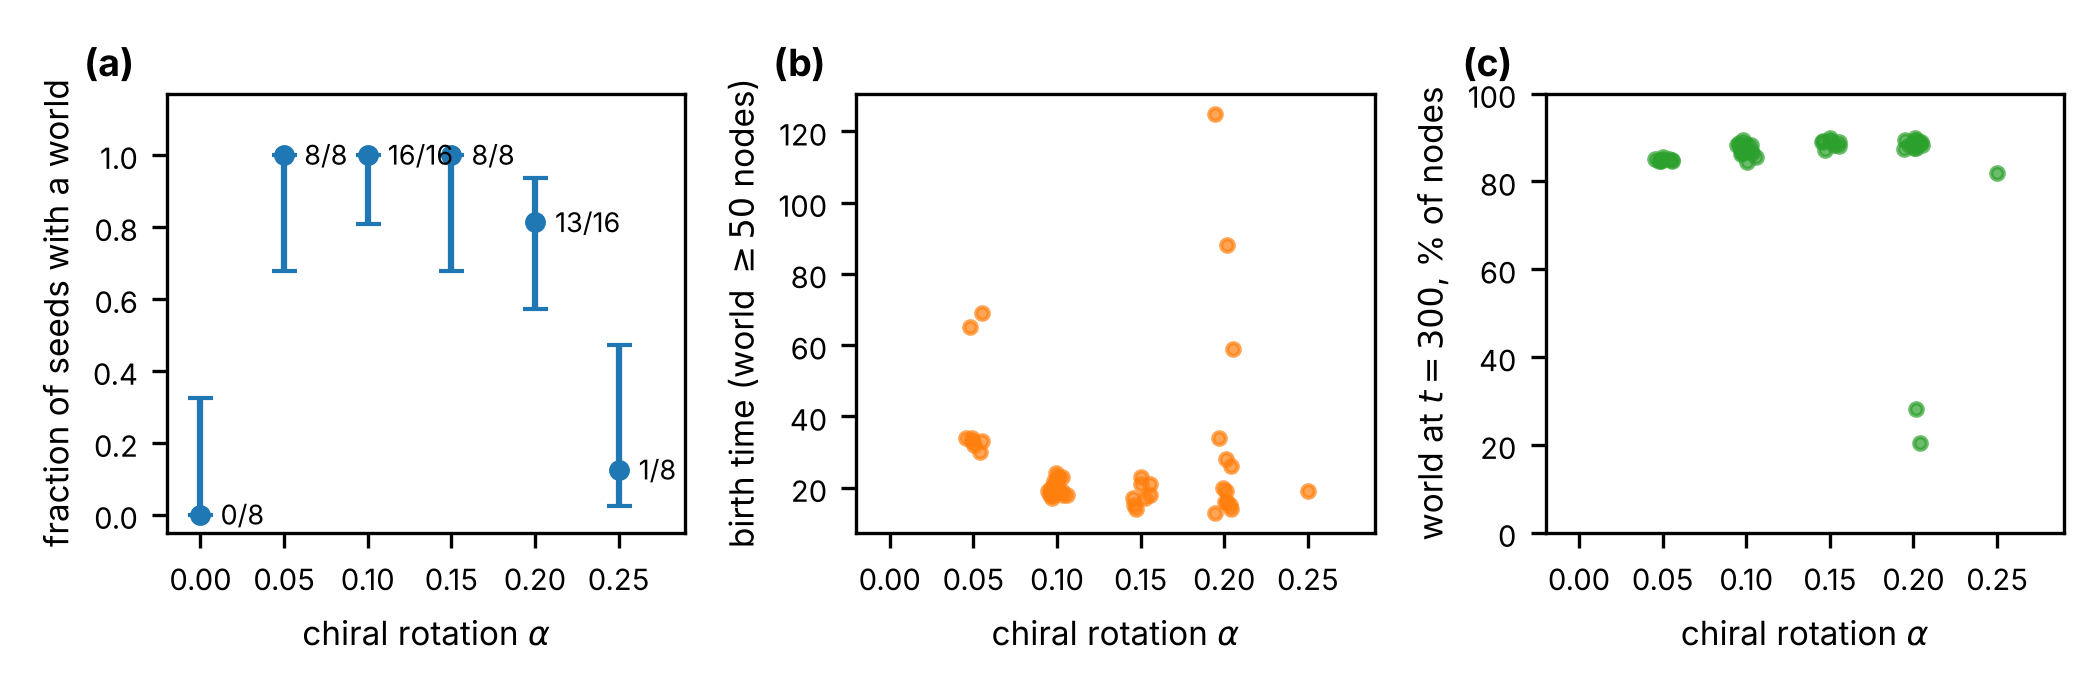
\includegraphics[width=\textwidth]{fig_birth}
\caption{Birth of a world versus chiral rotation ($\sz=3.0$, $h=0.30$, $L=16$, $T=300$; $\alpha=0$ to $T=100$). (a) Fraction of seeds with a world at the end, with 95\,\% Wilson intervals. (b) Birth time, when the largest world first reaches 50 nodes. (c) Size of the world at $t=300$. Points in (b), (c) are single seeds, jittered in $\alpha$.}\label{fig:birth}
\end{figure*}
\subsection{The budget threshold from linear stability}\label{sec:threshold}
Why does the world appear only near $\sz=3$? The intensity--$\psi$ sector of Eqs.~(\ref{eq:z})--(\ref{eq:psi}) answers this without scanning. At $\alpha=0$ the phases decouple (Sec.~\ref{sec:adler}): the conservation acts only radially, as a real factor multiplying $z_e$. About the homogeneous Matrix ($\rho=\sz$, $\psi=\psi_M$, flat loops), with $\rho$ and $\psi$ averaged over the links of a node,
\begin{equation}
\delta\dot\rho=(1-\hat K)\,(a\,\delta\rho+b\,\delta\psi),\qquad \delta\dot\psi=c\,\delta\rho+d\,\delta\psi, \label{eq:rhopsi}
\end{equation}
\begin{gather}
a=2\Big(-1-2\rho+3\beta\sqrt\rho+\frac{\lambda_c\psi_M}{2w^2}\Big),\nonumber\\
b=\frac{\rho\lambda_c}{w^2},\quad c=\frac{\deg\,\lambda_c}{4w^2},\quad d=-(3\psi_M^2-1),
\end{gather}
with $\deg=14$ and $\hat K$ the conservation kernel in Fourier space ($\hat K\to1$ as $k\to0$). For $k\neq0$ the factor $1-\hat K>0$ only sets the time scale, so the long waves are unstable exactly when
\begin{equation}
\det=ad-bc<0 .
\end{equation}
This gives $\szc=2.864$ at $h=0.36$, 2.787 at 0.33 and 2.755 at 0.30; without the coupling to $\psi$ ($b=c=0$, i.e.\ $a=0$ with $\psi$ held at $\psi_M$) it would be 2.658. In this sector the threshold depends neither on $\alpha$ nor on the range of $K$. For $h>2/(3\sqrt3)\approx0.385$ the Matrix minimum $\psi_M$ disappears (spinodal of $\psi$) and the world is everywhere, as observed at $h=0.39$ (Sec.~\ref{sec:islands}).

\emph{Check.} We compute the leading eigenvalue of the Jacobian of the full model in this sector (matrix-free directional derivatives and ARPACK) at $\alpha=0$, on $L=16$ and 32 [r453]. The criterion was set before the computation: the sign must change between $\sz=2.80$ and 2.93 at $h=0.36$ and between 2.70 and 2.81 at $h=0.30$. On the lattice the crossing lies lower, at 2.707 ($L=16$) and 2.822 ($L=32$) for $h=0.36$, and 2.647 and 2.726 for $h=0.30$ (Fig.~\ref{fig:threshold}). The shift scales as $1/L^2$, because the smallest wave number is $2\pi/L$ and the conservation factor is $\propto k^2$; assuming this law, the extrapolation $L\to\infty$ from the two sizes gives 2.860 and 2.752, within 0.005 of the derived values (two sizes fix the extrapolation but do not test the $1/L^2$ law itself). Below the threshold the fastest mode has a finite wavelength, about 16 links at $\sz=2.5$ on both $L=16$ and 32; it depends weakly on the range of the kernel (10.7, 16, 18.5 links at $n=25$, 100, 400, $\approx n^{0.2}$). This is a scale of domains of the field, not the lattice spacing; without the conservation law it would not exist, so it is partly set by hand.

\emph{What the threshold explains.} The base point $\sz=3.0$ lies just above $\szc$: the Matrix is linearly stable in this sector, and a world must nucleate. In the scan of Sec.~\ref{sec:birth} ($h=0.30$, $\szc=2.755$) all three budgets 2.85--2.95 are above the threshold, and the system is bistable---a world takes almost everything or does not form. At $\sz=3.45$ the Matrix is deep in the stable region and no nucleus appears. The upper edge of the budget window (between 3.0 and 3.45) is not derived. The boiling that seeds worlds at $\alpha>0$ is not this instability: it lives in the phase sector, Sec.~\ref{sec:adler}.


\begin{figure*}[t]
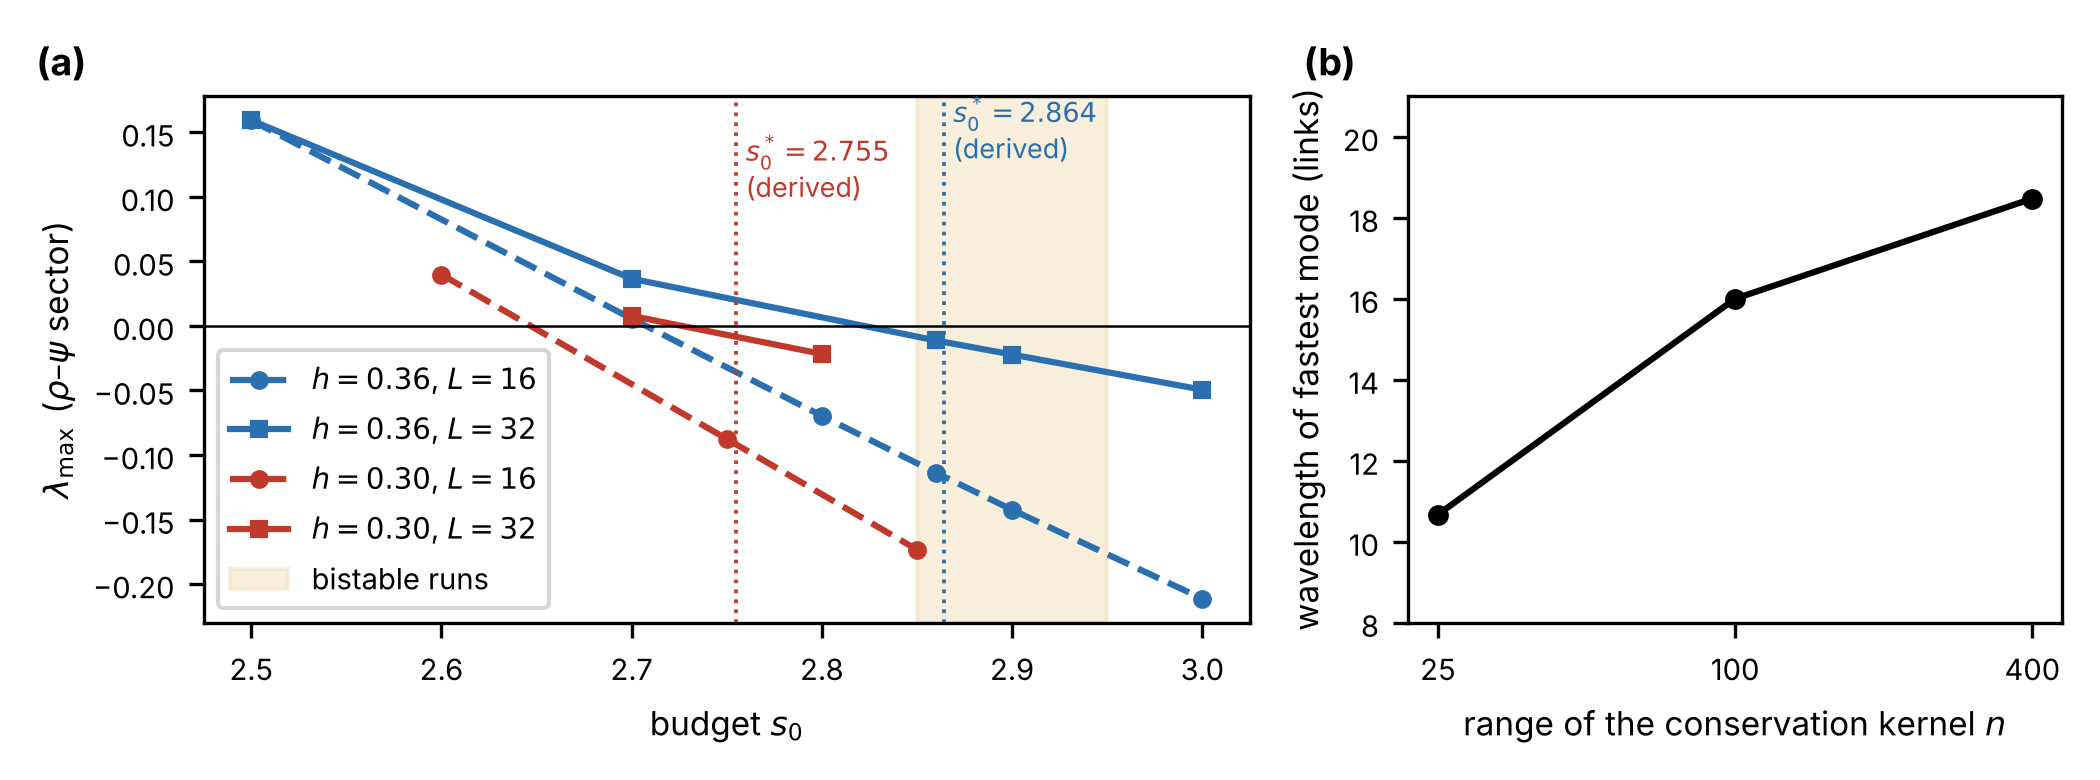
\includegraphics[width=\textwidth]{fig_threshold}
\caption{Budget threshold of the Matrix ($\alpha=0$). (a) Leading eigenvalue of the full Jacobian in the $\rho$--$\psi$ sector on $L=16$ and 32; dotted lines, the derived $\szc$; shaded, the budgets of the bistable scan of Sec.~\ref{sec:birth}. (b) Wavelength of the fastest mode below the threshold ($\sz=2.5$, $h=0.36$, $L=32$) versus the range $n$ of the conservation kernel $K=P^n$.}\label{fig:threshold}
\end{figure*}
\subsection{Loop phases: an Adler equation}\label{sec:adler}
Since the conservation law acts only on $|z_e|$, the phases $\theta_e=\arg z_e$ are free, and only loop phases $\Phi_q=\sum_{j\in q}S_j\theta_j$ ($S_j=\pm1$ the orientation of link $j$ in loop $q$) are physical. In the homogeneous Matrix ($|z_e|=A=\sqrt{\sz}$, $\psi=\psi_M$) the weight $\chi(\psi_M)\approx0.02$ makes the $\varepsilon_0$ term small, and Eq.~(\ref{eq:z}) reduces to
\begin{equation}
\dot\theta_e=\frac{2\beta A}{k_e}\sum_{q\ni e}\Big[\alpha\cos\Phi_q-\frac{S_e}{a}\sin\Phi_q\Big],\label{eq:adler}
\end{equation}
an Adler equation for coupled loops: the sine term locks loops flat, the cosine term, set by chirality, drives them. Two consequences follow directly. (i) The homogeneous state does not stand but rotates with $\omega=2\alpha\beta A$; numerically $\omega=1.126$ at $\alpha=0.25$, $\sz=3$, equal to the formula to $10^{-15}$. (ii) A loop with unbalanced orientations, $\sigma_q=\sum_jS_j\neq0$, drifts unless the locking term can hold it.

\emph{Collective, not single-loop, locking.} A mean-field estimate for one loop with $\sigma=2$ gives locking for $\alpha<\tfrac12\sum_j1/(ak_j)=0.22$--0.33, i.e.\ a step in the locked fraction from 1 to $\approx0.67$ (only $\sigma=0$ loops left). We test it in the full model ($h=0.36$, flat start with phase noise $10^{-3}$, $t=0$--25; a loop is locked if its phase moves by less than 0.5 rad over $t=10$--15 and 20--25). On $L=16$ with 8 seeds per point [r452V] the locked fraction of $\sigma=2$ loops is $1.000$, $0.994\pm0.002$, $0.912\pm0.003$, $0.925\pm0.006$, $0.944\pm0.005$, $0.940\pm0.003$, $0.922\pm0.004$ and $0.880\pm0.005$ at $\alpha=0$, 0.05, 0.1, 0.15, 0.2, 0.25, 0.3 and 0.4. There is no step (Fig.~\ref{fig:loops}): the loops lock collectively, and the single-loop picture fails. Drift sets in already at $\alpha=0.05$--0.1. On $L=8$ (2 seeds) all loops stayed locked up to $\alpha=0.15$ [r452]; that was a small-box effect, as for the threshold in Sec.~\ref{sec:threshold}: the long waves, which grow fastest at $\alpha>0$ [r422], do not fit into $L=8$. The static twist $\langle1-\cos\Phi\rangle$ at $\alpha=0.05$ is 0.022 on $L=16$ against 0.003 on $L=8$. In the window $\alpha=0.1$--0.2 a world nucleates before $t=25$ in every seed, so we split the loops by $\psi$ at their four nodes [r452G]. Before any world exists ($t=10$--15) the loops of the Matrix alone give 0.959, 0.941 and 0.944 at $\alpha=0.1$, 0.15 and 0.2: the Matrix drifts by itself. Once a world is present ($t=20$--25), all loops inside it are locked (1.000), while the remnant Matrix next to it unlocks much more strongly (0.28 at $\alpha=0.1$, 0.72 at 0.15). The world removes the twist from its own loops and pushes it into the surrounding Matrix, as the static snapshots below also show. That drift begins at the left edge of the birth window suggests that drifting loops are the boiling that seeds worlds; this is a hypothesis.

\emph{A candidate for the right edge.} Inside a world $\chi\approx1.15$, and twisted loops cost energy through the $\varepsilon_0$ term. On final states of worlds grown on field lattices, loops inside the world are nearly untwisted (0.0025--0.0048 at $\alpha=0.1$, 8 seeds; 0.013--0.018 at 0.25, 6 seeds), while the Matrix next to the world is strongly twisted (0.26--0.69, against 0.09 without a world): the world expels the twist rather than removing it [r452B]. The cost of the residual twist inside the world, per node, is 0.15 at $\alpha=0.1$ and 0.47 at 0.25, compared with the gain of the $\psi$ transition $\Delta V\approx0.71$ at $h=0.36$. Extrapolated as $\alpha^{1.25}$, the cost equals the gain at $\alpha\approx0.34$. The measured edge at $h=0.30$ lies between 0.2 and 0.25 (Sec.~\ref{sec:birth}), and at $h=0.36$ worlds still form at $\alpha=0.25$ (Sec.~\ref{sec:islands}). The estimate has the right order and the right trend with $h$, but it uses two points, mixes $h=0.30$ and 0.36, and neglects the $\lambda_c$ and $\kappa$ terms of the gain. We state it as a hypothesis: the right edge of the window is where the price of untwisting loops eats the gain of the world. Its testable form is $\alpha_c\propto\Delta V^{0.8}$.

\begin{figure*}[t]
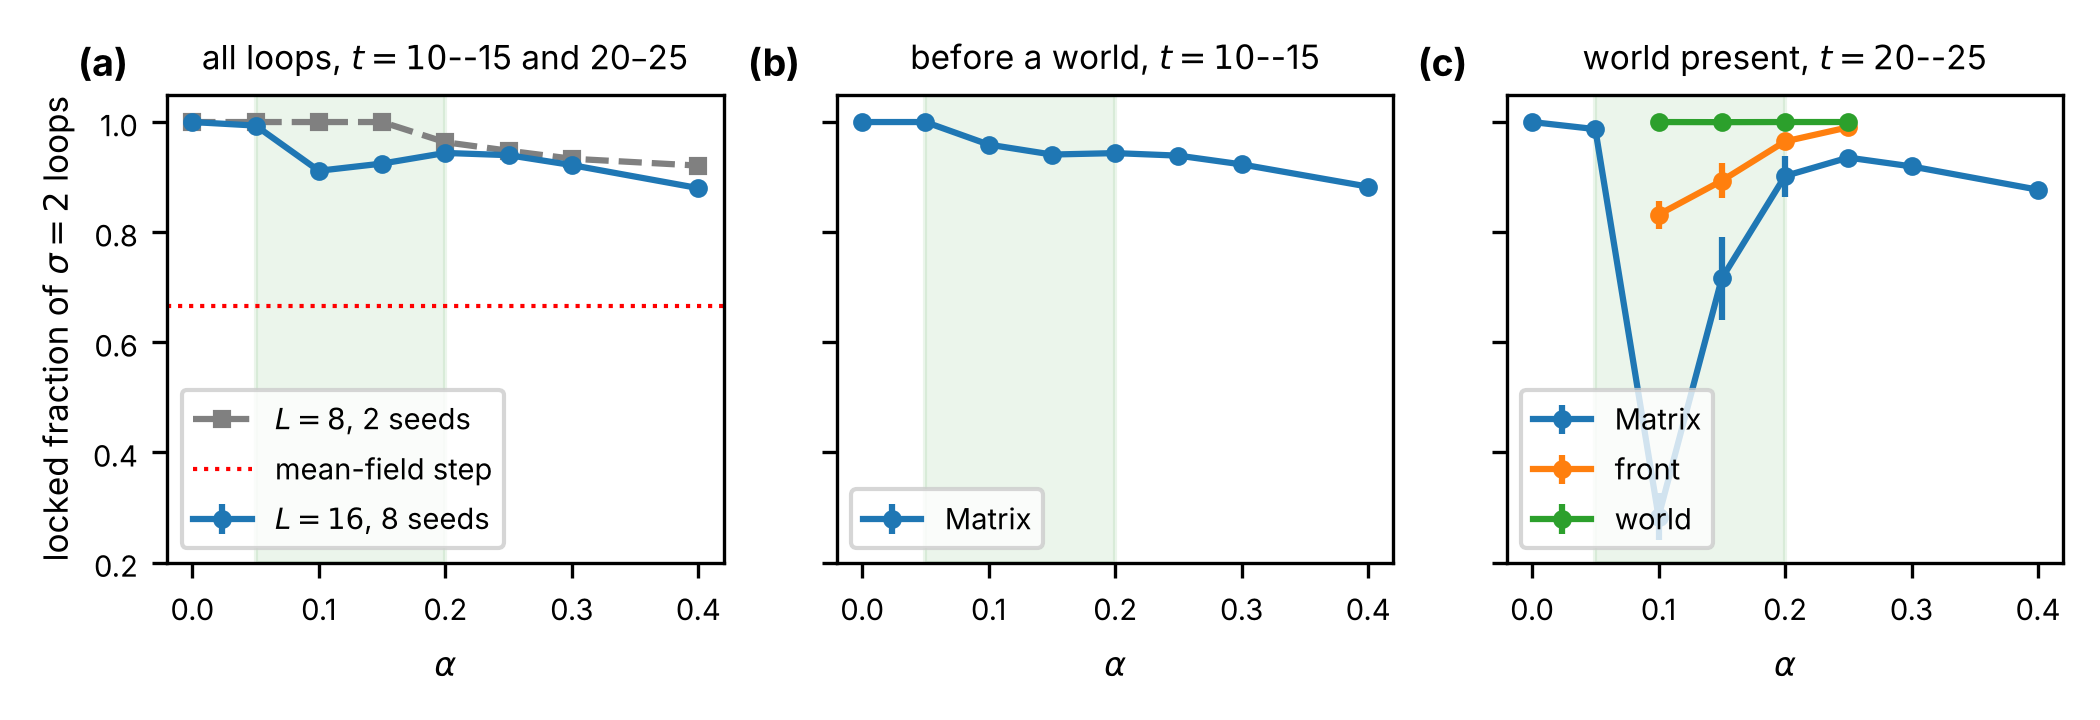
\includegraphics[width=\textwidth]{fig_loops}
\caption{Locking of loop phases ($h=0.36$, $L=16$, 8 seeds; shaded, the birth window of Fig.~\ref{fig:birth}). (a) Locked fraction of $\sigma=2$ loops; dashed, the earlier $L=8$ runs; dotted, the single-loop mean-field step. (b) Matrix loops before any world exists. (c) After a world has formed, loops split by $\psi$ at their nodes into Matrix, front and world. Error bars, standard error over seeds.}\label{fig:loops}
\end{figure*}
\subsection{Finite islands}\label{sec:islands}
A world that fills the whole box says nothing about whether a world can be \emph{finite}. We ask two questions: can a finite world stand inside a hostile medium, and does the living Matrix produce finite worlds by itself?

\emph{A planted patch.} We plant a ball of radius 8 of ordered links into a frustrated, chaotic network ($L=24$) and conserve the budget separately inside and outside the patch [r420B]. A world forms in 5 of 8 seeds, always inside the patch ($r_{\max}=6.5$--$6.7$, 800--1160 nodes), and stays unchanged from $t=100$ to 300; the control without frustration gives a world over the whole box in 8 of 8. Part of the wall in this test is built in by the separate conservation, so we use it only as an existence proof.

\emph{Islands in the living Matrix.} Without any planted structure, at $\alpha=0.25$, $h=0.36$, $\sz=3.0$, $L=16$, $T=600$ [r425]. An \emph{island} is defined before the runs: the largest world has between 50 nodes and 40\,\% of the lattice at $t=600$, the surrounding Matrix stays alive ($\rho>2.5$), and its size changes by less than 20\,\% between $t=300$ and 600. Of 24 seeds (Fig.~\ref{fig:islands}a), 7 give a stable island ($29\pm9\,\%$; 3--32\,\% of the lattice), 8 a world over the whole box, 8 nothing, and 1 an island that still grows. The first 16 seeds (4 islands) and the later 8 (3 islands) agree. At $h=0.39$, above the spinodal of $\psi_M$ ($h>2/3\sqrt3=0.385$), the world fills the box in 8 of 8. Islands live in a narrow band of $h$: 2/8 at $h=0.35$, 3/8 at 0.37, none at 0.30, 0.33 and 0.39 [r425V] (all on $L=16$; see Sec.~\ref{sec:birth} for $L=24$).

Which of the three outcomes a seed gives is not a matter of noise: it is set by the arrow field, as Sec.~\ref{sec:tau} shows directly. We therefore read 7/24 as the fraction of arrow fields that produce a finite world at this point, not as a nucleation probability. Limitations: one box size ($L=16$), one $\alpha$.

\subsection{The arrow of time fixes the place of birth}\label{sec:tau}
Sec.~\ref{sec:birth} hinted that the arrows, not the noise, set the clock of birth. For islands (Sec.~\ref{sec:islands}) we test the place. The arrow field $\tau$ and the initial noise come from separate random generators, so we can keep $\tau$ and change the noise.

\emph{Test.} We take the four arrow fields that gave an island in [r425] and run each with 8 new noise realizations ($\alpha=0.25$, $h=0.36$, $\sz=3.0$, $L=16$, $T=600$; 32 runs) [r449B]. Two islands occupy the same place if their overlap $|A\cap B|/\min(|A|,|B|)$ is at least 0.5 and above the 95th percentile of the overlap under 2000 random periodic shifts of one mask. The criterion was fixed before the runs: confirmed if at least 70\,\% of the islands sit at the original place, refuted if at most 20\,\%.

\emph{Result.} An island forms in all 32 runs, and in all 32 at the original place (Fig.~\ref{fig:islands}b): overlap 0.95--1.0, 0.92--1.0, 0.99--1.0 and 0.94--1.0 for the four arrow fields, against null levels of 0.18--0.66. Island sizes are reproducible within an arrow field (135 to $\approx1190$ nodes between fields). The place also does not move when $h$ changes from 0.35 to 0.37 (overlap 0.92--1.0, 6 seeds) [r449]. Because a result this clean can hide a test that cannot fail, we repeated one arrow field with ten times larger initial noise in $\psi$: the island again forms in 8 of 8 runs, at the same place.

A first version of this control also multiplied the noise in the link amplitudes. That raised the mean intensity by $\approx2\,\%$, and no island or world formed in 8 of 8 runs. This side result shows how close the islands sit to the edge of the budget window (compare Sec.~\ref{sec:birth}, $\sz=3.45$).

\emph{What sets the place.} The island does not simply sit where $\tau$ is steepest: in three arrow fields it does (percentile of $|\nabla\tau|$ 0.97--1.0), in the fourth it sits where $\tau$ is flattest (0.03--0.08). The value of $\tau$ and its Laplacian show no pattern. The place of a world is thus written in the frozen orientation field, but we do not yet know which feature of it is read.


\begin{figure*}[t]
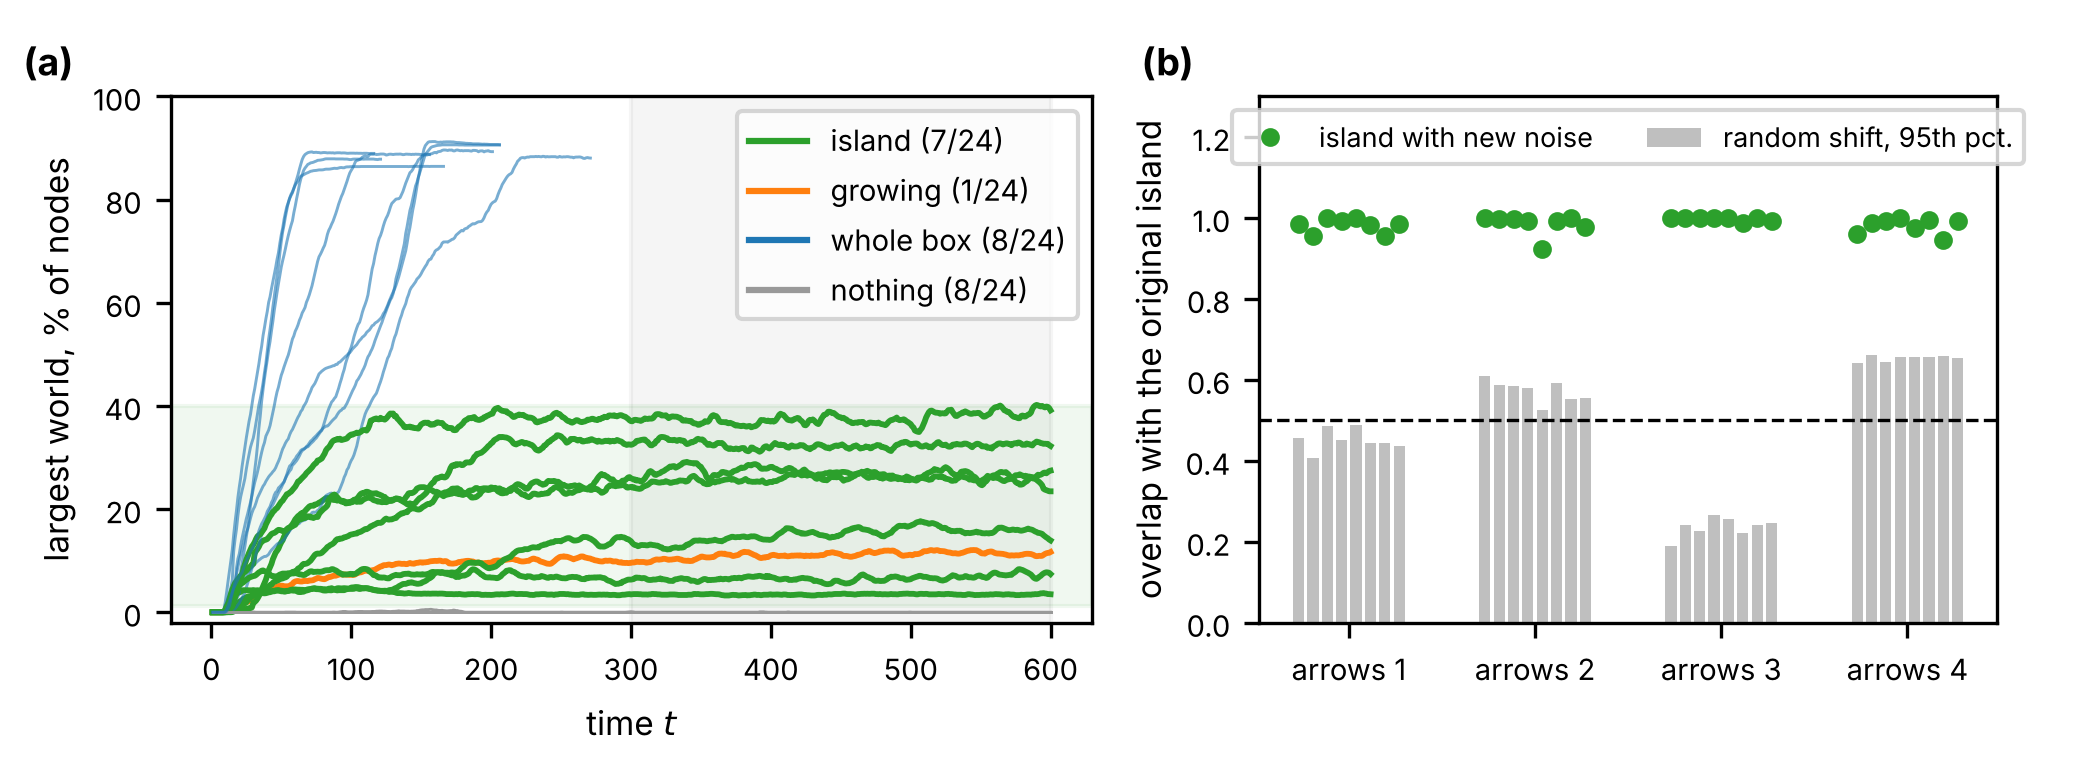
\includegraphics[width=\textwidth]{fig_islands}
\caption{Finite islands and their place ($\alpha=0.25$, $h=0.36$, $\sz=3.0$, $L=16$). (a) Largest world versus time for 24 seeds, classified by the criterion fixed before the runs (green band: island size range; grey: interval $t=300$--600 where stability is tested). (b) Overlap of the island grown with new noise with the original island, for the four arrow fields that gave islands (8 runs each); grey bars, the 95th percentile of the overlap under random periodic shifts; dashed, the threshold 0.5.}\label{fig:islands}
\end{figure*}
\subsection{Worlds on lattices grown from a field}\label{sec:lattices}
The Kuhn lattice is put in by hand. Can it be replaced by a lattice that grows from a field, with the defects such growth leaves?

\emph{Growing the lattice.} We use a phase-field crystal (conserved Swift--Hohenberg) at $\bar\psi=-0.30$, whose ground state is body-centred cubic (bcc); nodes are the maxima of the field. Two nodes are joined if their Voronoi cells share a face, and the loops are the four-link cycles of the Delaunay tetrahedra. For bcc this rule gives exactly the 14 neighbours of the Kuhn lattice, and among cubic lattices only bcc gives tetrahedral cells [r464]. A generic module for such lattices reproduces the Kuhn dynamics to $2\times10^{-15}$. Quenching or slowly cooling a box of 13 bcc cells (the size of $L=16$) gives a glass in 16 of 16 runs: the cooling ramp crossed the spinodal of the liquid at $\varepsilon=3\bar\psi^2=0.27$ [r447]. Inside the metastable window $0.22<\varepsilon<0.27$ the crystal can only grow from a nucleus. A bcc ball of two cells at a random orientation grows into a crystal over the whole box in 8 of 8 runs (88--100\,\% bcc by common-neighbour analysis), against no crystal in 8 of 8 runs without a nucleus [r448]. Since a rotated crystal does not fit the periodic box, the mismatch collects into a sheet or lines of defects; 0--5\,\% of the nodes have a coordination other than 14 (a stricter count than the defect fraction by common-neighbour analysis used below).

\emph{Worlds on grown lattices.} On these 8 lattices, with their natural defects ($\alpha=0.1$, $h=0.30$, $\sz=3.0$, $T=300$), a world forms in 8 of 8 runs, born at $t=22$--24 and taking 85--87\,\% of the nodes, as on the Kuhn lattice [r450] (Fig.~\ref{fig:lattices}). Defect nodes (0--12\,\% by common-neighbour analysis) are taken by the world as readily as bcc nodes (56--94\,\% against 85--88\,\%), and the outcome does not depend on the defect fraction. The chain field $\to$ lattice $\to$ Matrix $\to$ world closes in three dimensions, under one condition we put in by hand: a single nucleus in the metastable window. Limitations: one box size; the field that grows the lattice is not the field of the model.


\begin{figure*}[t]
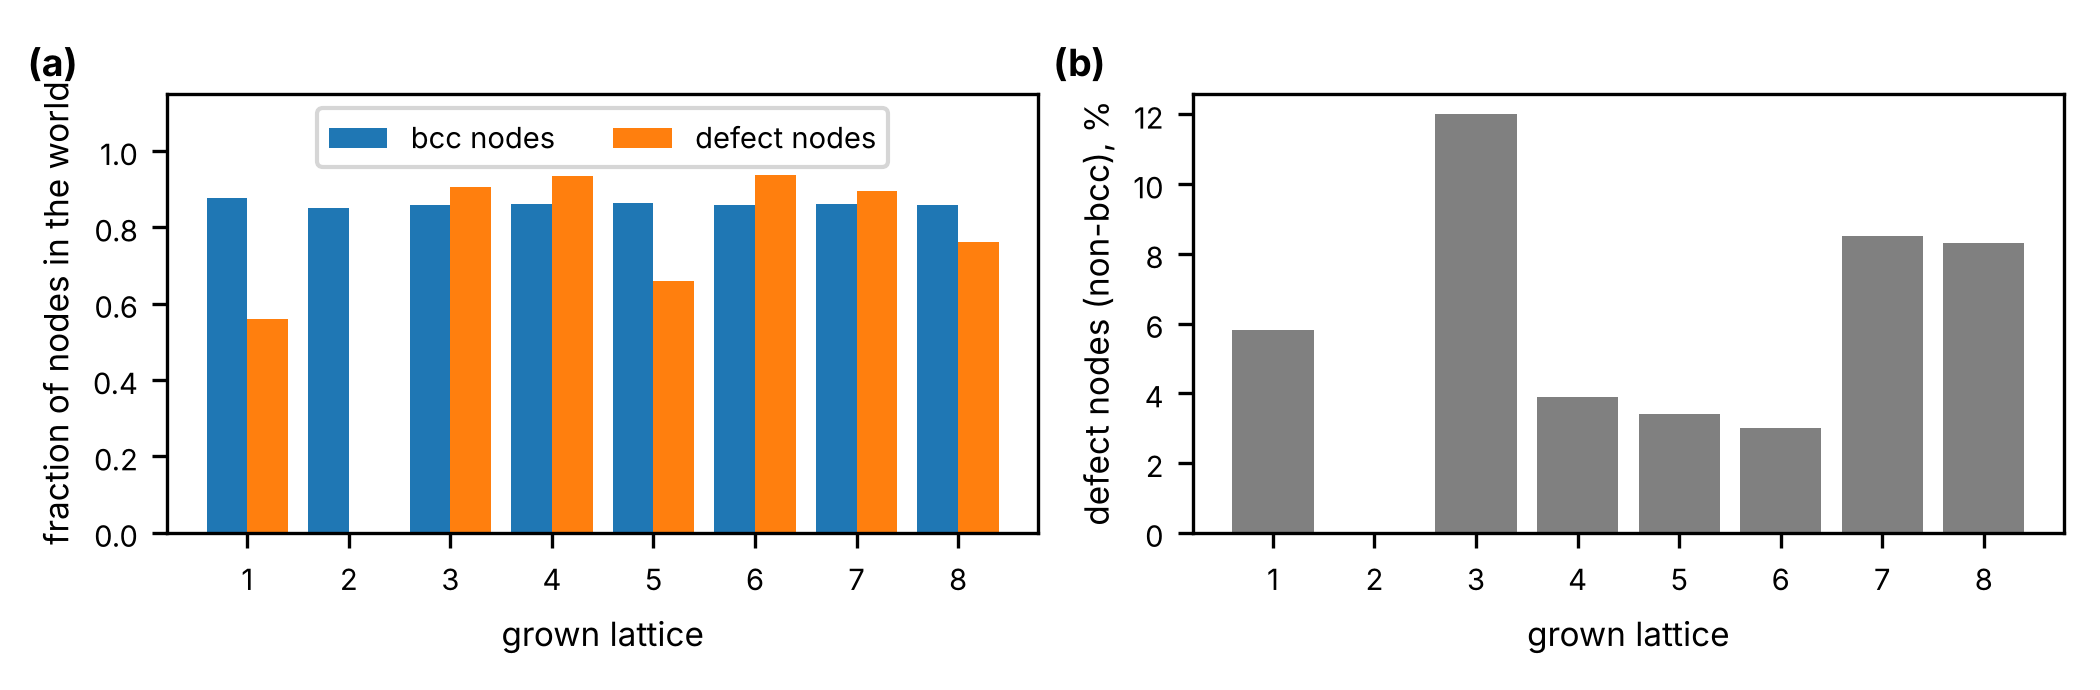
\includegraphics[width=\textwidth]{fig_lattices}
\caption{Worlds on lattices grown from a phase-field crystal ($\alpha=0.1$, $h=0.30$, $\sz=3.0$, $T=300$). (a) Fraction of bcc nodes and of defect nodes taken by the world on each of the 8 lattices (lattice 2 has no defects). (b) Fraction of defect nodes (common-neighbour analysis) in each lattice.}\label{fig:lattices}
\end{figure*}
\subsection{Response of the Matrix near the threshold}\label{sec:critical}
The threshold of Sec.~\ref{sec:threshold} has a second consequence. Near $\szc$ the homogeneous Matrix is soft, and a local perturbation should spread further. We test this with a static source.

\emph{Linear theory.} Linearizing Eqs.~(\ref{eq:z})--(\ref{eq:psi}) about the homogeneous Matrix ($\rho=\sz$, $\psi=\psi_M$, flat loops) gives the reduced system of Sec.~\ref{sec:threshold},
\begin{equation}
\delta\dot\rho=(1-\hat K)\big[a\,\delta\rho+b\,\delta\psi+\mu(x)\big],\qquad \delta\dot\psi=c\,\delta\rho+d(k)\,\delta\psi, \label{eq:lin}
\end{equation}
with $d(k)=d_0-\kappa' k^2$ at small $k$ ($\kappa'$ the effective gradient stiffness of $\psi$ on the lattice) and $\mu(x)$ an external source acting on link intensities. In the static state the factor $1-\hat K$ cancels for every $k\neq0$ (it only removes the uniform mode), so the conservation kernel does not shape the response. Solving for $k\neq0$,
\begin{equation}
\delta\rho(k)=\frac{\mu}{|a|}+\frac{\mu\,bc/|a|}{\det+|a|\kappa' k^2},\qquad \det=a d_0-bc,
\end{equation}
i.e.\ a contact term plus a screened (Yukawa) halo of the \emph{same sign} as the source, with range $\xi^2=|a|\kappa'/\det$. Since $\det\to0$ at $\szc$, $\xi\propto(\sz-\szc)^{-1/2}$: $\xi=4.7$, 2.9, 2.4 lattice spacings at $\sz=2.9$, 3.0, 3.15. Only a \emph{deficit} of budget ($\mu<0$) gives a depleted halo. A $1/r$ halo would require $\sz-\szc\lesssim10^{-4}$.

\emph{Test.} We add $+\mu z_e$ to the links within distance 1 of a node, with the same conservation law, and run to the stationary state ($T=120$, $|\mu|=0.2$). Five arms, 8 seeds each: $\sz=2.9$, 3.0, 3.15 at $\mu=+0.2$ and $L=16$; $\sz=3.0$ at $\mu=-0.2$; $\sz=2.9$ at $L=24$. The sign of the halo equals the sign of $\mu$ in 8 of 8 seeds in every arm [r470].

\emph{Comparison without free parameters.} A Yukawa fit $A\,e^{-r/\xi}/r+C$ to the halo is ill-conditioned: the fitted $\xi$ depends on the fitting window (at $\sz=2.9$, $L=16$: 3.2, 7.0 and 9.0 for $r\ge2$, 3, 4). We therefore compare with the exact linear response of the same lattice instead. We apply the Jacobian of the full model, Eqs.~(\ref{eq:z})--(\ref{eq:psi}), at the homogeneous Matrix, solve $J\,\delta x=-\mu\,\partial_\mu F$ by GMRES (relative residual $<3\times10^{-7}$) on the same box, with the same arrows and the same source position, and compare $\delta\rho(r)$ relative to the box mean [r470G]. Nothing is fitted. The shape agrees to within 1\,\% of $\delta\rho(2)$ for $2\le r\le L/2-2$ in all 40 runs, once a single overall amplitude is allowed (Fig.~\ref{fig:critical}). Without any adjustment the amplitude ratio data/theory is 0.89 ($\sz=2.9$, $L=16$), 0.90 ($L=24$), 0.92 (3.0) and 0.94 (3.15) for $\mu=+0.2$, and 1.14 for $\mu=-0.2$; the spread between seeds is below 0.4\,\%. The deviation changes sign with $\mu$, as expected of the first nonlinear correction. Fitting the exact linear profile with the same Yukawa form reproduces the window dependence of $\xi$; it is a property of the fit in a finite box, not of the data.

The halo is therefore the linear response of a lattice near its stability threshold, and its range grows as $\sz\to\szc$. Limitations: $\alpha=0$; one source shape; boxes $L\le24$, smaller than or comparable to $\xi$ near the threshold. The world itself does not hold the Matrix at the threshold: it drives $\rho_M$ below $\szc$ and the Matrix dies there. A mechanism that keeps the Matrix critical is an open question (Sec.~\ref{sec:outlook}).

\begin{figure*}[t]
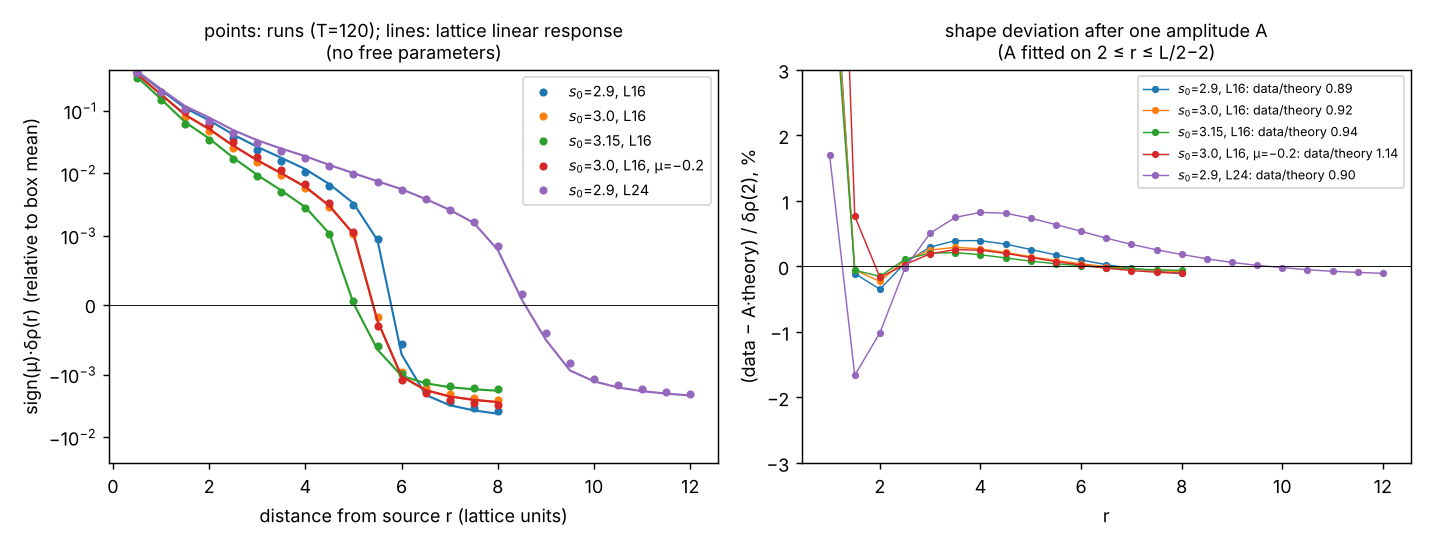
\includegraphics[width=0.9\textwidth]{fig_critical}
\caption{Halo around a static source. Left: $\mathrm{sign}(\mu)\,\delta\rho(r)$ relative to the box mean; points, stationary runs; lines, exact linear response of the same lattice, no free parameters. Right: deviation of the shape after one overall amplitude, in units of $\delta\rho(2)$.}\label{fig:critical}
\end{figure*}


\section{Relation to known approaches}\label{sec:related}
\emph{Emergent geometry from networks.} Quantum graphity~\cite{Konopka2006,Konopka2008} and causal dynamical triangulations~\cite{Ambjorn2004} also start without a given space. In quantum graphity the graph itself is dynamical and cools into a low-connectivity, lattice-like phase; in our model the lattice is fixed (or grown from a separate field, Sec.~\ref{sec:lattices}), and what emerges is not the geometry but a phase of the fields on it. Our model is classical and dissipative, and makes no claim about quantum gravity.

\emph{Phase-field crystals and nucleation.} The lattices of Sec.~\ref{sec:lattices} are grown with the standard phase-field crystal (conserved Swift--Hohenberg) model~\cite{Swift1977,Elder2002,Elder2004}; the glass after a quench and the growth from a nucleus in the metastable window are its known behaviour, which we reproduce rather than discover. The birth of a world is first-order nucleation (see Ref.~\cite{Oxtoby1992} for a review): above $\szc$ the Matrix is metastable, and a world needs a nucleus. In the classification of Ref.~\cite{Hohenberg1977} the $\rho$--$\psi$ sector of Eq.~(\ref{eq:rhopsi}) is model C: a conserved density (the link intensity) coupled to a non-conserved order parameter ($\psi$). The threshold $\szc$ of Sec.~\ref{sec:threshold} is the spinodal of this coupled system, and the halo of Sec.~\ref{sec:critical} is its static response near the spinodal. What is specific here is that the nucleus is not thermal: the noise is frozen into the arrow field, so the place of birth is deterministic (Sec.~\ref{sec:tau}), as in heterogeneous nucleation on quenched disorder.

\emph{Phase locking.} Equation~(\ref{eq:adler}) is a network of Adler equations~\cite{Adler1946}, i.e.\ a Kuramoto-type model~\cite{Kuramoto1984,Acebron2005} on loops rather than on oscillators, with a frustration set by the orientations $S_j$. Since the phases live on links and lock on loops, it belongs to the recently studied synchronization of signals on the edges of simplicial complexes, where phases on edges are coupled through faces~\cite{Millan2020}. The collective unlocking without a single-loop step (Sec.~\ref{sec:adler}) is the expected behaviour of such coupled systems; the new element is that unlocking is coupled to the budget and to $\psi$, so that it can seed a phase transition.

\emph{Non-reciprocal media.} The chiral factor $1+i\alpha$ makes the link interaction non-reciprocal. Non-reciprocal interactions are known to produce time-dependent phases and to change the nature of transitions~\cite{Fruchart2021}; here they turn a stable Matrix into a boiling one, which nucleates worlds.

\emph{Response near a spinodal.} The halo of Sec.~\ref{sec:critical} is the Ornstein--Zernike form of a linear response near a spinodal, with a correlation length $\xi\propto(\sz-\szc)^{-1/2}$. We do not claim a new mechanism; the point is that the lattice reproduces it exactly, which makes the halo a calibrated probe for later work.

\section{Negative results}\label{sec:neg}
Several natural expectations failed. We list them because they constrain the model and show that it was not tuned to the answer (Table~\ref{tab:neg}).

\begin{table*}[t]
\caption{Negative results. All runs: Kuhn lattice, $L=16$, 8 seeds per point unless stated.}\label{tab:neg}
\begin{ruledtabular}
\begin{tabular}{p{0.30\textwidth}p{0.52\textwidth}l}
Expectation & Outcome & Ref.\\
\hline
Rules of Part~I work in 3D as they are & no world in 12 runs, $\sz=2.5$--4.25, $\alpha=1$ (default of Part~I) & [r351]\\
A world forms at strong rotation & no world at $\alpha=0.3$--0.7 (1 seed each); window closes at 0.2--0.25 ($L=16$); on $L=24$ still 4/8 at 0.25, larger $\alpha$ not run & [r355], [r375], [r479]\\
The Matrix has an intrinsic length (Turing-like instability at finite $k$) & no: at $\alpha=0$ all modes decay, at $\alpha=0.1$ the longest waves grow fastest (8/8, 7/8) & [r422]\\
Birth is set by an effective temperature of the boiling & no: it does not separate points with and without births (9 points in $\alpha$, $\sz$) & [r423]\\
Birth is set by the depth $\bar\psi$ of the Matrix & no: shifting $\bar\psi$ by $h$ gives the opposite of the prediction (8/8 instead of $\le2/8$) & [r424]\\
A patch of Matrix lives in a loop-free chaotic network & no world in 8/8; the patch empties in 6/8 & [r420]\\
Single-loop mean field gives the right edge of the window & no step in the locked fraction; drift is collective and starts at $\alpha\approx0.1$; $L=8$ hid it & [r452], [r452V]\\
A lattice crystallizes from a random field in a box of $L=16$ & glass in 16/16 (ramp crossed the spinodal); bcc only from a nucleus & [r447], [r448]\\
Coupling constants per link select the dimension; worlds in 4D & 4D Matrix survives, but no world by $t=50$ in 16/16 (a late world in 3/8) & [r461]--[r463]\\
A simple budget model predicts where a growing front stops ($x\approx0.3$) & fronts stop at $x=0.71$--0.93 & [r458]\\
\end{tabular}
\end{ruledtabular}
\end{table*}

\emph{Limits of the model.} The lattice (or the nucleus that grows it), the arrows $\tau$ and the chiral rotation $\alpha$ are put in by hand. The windows in the parameters are narrow: $\alpha=0.05$--0.2 at $h=0.30$, islands only at $h=0.35$--0.37 on $L=16$; on $L=24$ the upper edge softens and islands appear also at $h=0.30$ (4 of 8 seeds at $\alpha=0.25$ to $T=600$), so the windows depend on the box size. The dynamics is first order in time, so the Matrix carries no waves and no finite signal speed. The boxes are small ($L\le24$), and the $L=8$ result of Sec.~\ref{sec:adler} shows how a small box can mislead. Every statement above is about a classical toy model.

\section{Outlook}\label{sec:outlook}

The results raise five questions, each with a test that can fail.

\emph{What keeps the Matrix near its threshold?} The halo of Sec.~\ref{sec:critical} is long-ranged only near $\szc$, but a world drives the surrounding Matrix below the threshold, where it dies. A Matrix that stays near $\szc$ by itself---through an inflow of budget, a feedback from the world, or a slow drift of $h$---would turn the screened halo into a long-ranged one. In our runs no such mechanism appears. A depleted halo forms only around a deficit of budget that we impose by hand ($\mu<0$); it is not a gravitational effect.

\emph{What sets the right edge of the window?} The hypothesis of Sec.~\ref{sec:adler}, that the edge is where the cost of untwisting loops eats the gain of the world, predicts $\alpha_c\propto\Delta V^{0.8}$. Measuring the edge at several $h$ on $L=24$ tests it directly.

\emph{Which feature of the arrows is read?} The place of an island is written in the frozen field $\tau$ (Sec.~\ref{sec:tau}), but neither its gradient, its value nor its Laplacian predicts it. A linear analysis of the Matrix with a given $\tau$, looking for the most unstable local mode, is the natural next step.

\emph{Can the model grow its own lattice?} The lattices of Sec.~\ref{sec:lattices} come from a separate field and need a nucleus. A lattice that grows from the order parameter of the Matrix itself would remove one of the three ingredients put in by hand.

\emph{Waves and dimension.} The dynamics is first order in time, so there is no signal speed; second-order dynamics is required before any statement about light or gravity. In four dimensions the Matrix survives but worlds form late or not at all (Table~\ref{tab:neg}); whether three dimensions is selected, and not merely chosen, remains open.

% (478) monopole motion, added 24.11 by author's decision; preliminary, no numbers
The model also hosts a stable holonomy monopole: a tetrahedron around which the link phases wind by $2\pi$. It is pinned by the lattice. An estimate, not yet tested numerically, suggests that under a strong enough applied flux it moves with friction and a threshold, as a first-order (overdamped) defect at $\alpha=0$. Its law of motion, the interaction of monopole pairs and possible inertia at $\alpha>0$ are left for separate work.

\begin{acknowledgments}
We thank an independent reader for a critical review of a draft of this paper. Numerical work and drafting were assisted by an AI model (Claude, Anthropic); all results were checked by the author.
\end{acknowledgments}

\begin{thebibliography}{99}
\bibitem{Batrukh2026v1} V. Batrukh, Self-boiling lattice of complex links: finite domains, elastic coexistence and a massless gauge mode in a 2D toy model of cosmogenesis, Zenodo (2026), \href{https://doi.org/10.5281/zenodo.23838333}{doi:10.5281/zenodo.23838333}.
\bibitem{Batrukh2026alice} V. Batrukh, Alice strings read soft photons: $Z_2$ defects of an SO(5) order parameter on a lattice of links, Zenodo (2026), \href{https://doi.org/10.5281/zenodo.24226818}{doi:10.5281/zenodo.24226818}.
\bibitem{Deser1984} S. Deser, R. Jackiw, and G. 't Hooft, Three-dimensional Einstein gravity: dynamics of flat space, Ann. Phys. \textbf{152}, 220 (1984).
\bibitem{Konopka2006} T. Konopka, F. Markopoulou, and L. Smolin, Quantum graphity, arXiv:hep-th/0611197 (2006).
\bibitem{Konopka2008} T. Konopka, F. Markopoulou, and S. Severini, Quantum graphity: a model of emergent locality, Phys. Rev. D \textbf{77}, 104029 (2008).
\bibitem{Ambjorn2004} J. Ambj{\o}rn, J. Jurkiewicz, and R. Loll, Emergence of a 4D world from causal quantum gravity, Phys. Rev. Lett. \textbf{93}, 131301 (2004).
\bibitem{Swift1977} J. Swift and P. C. Hohenberg, Hydrodynamic fluctuations at the convective instability, Phys. Rev. A \textbf{15}, 319 (1977).
\bibitem{Elder2002} K. R. Elder, M. Katakowski, M. Haataja, and M. Grant, Modeling elasticity in crystal growth, Phys. Rev. Lett. \textbf{88}, 245701 (2002).
\bibitem{Elder2004} K. R. Elder and M. Grant, Modeling elastic and plastic deformations in nonequilibrium processing using phase field crystals, Phys. Rev. E \textbf{70}, 051605 (2004).
\bibitem{Hohenberg1977} P. C. Hohenberg and B. I. Halperin, Theory of dynamic critical phenomena, Rev. Mod. Phys. \textbf{49}, 435 (1977).
\bibitem{Oxtoby1992} D. W. Oxtoby, Homogeneous nucleation: theory and experiment, J. Phys.: Condens. Matter \textbf{4}, 7627 (1992).
\bibitem{Adler1946} R. Adler, A study of locking phenomena in oscillators, Proc. IRE \textbf{34}, 351 (1946).
\bibitem{Millan2020} A. P. Mill\'an, J. J. Torres, and G. Bianconi, Explosive higher-order Kuramoto dynamics on simplicial complexes, Phys. Rev. Lett. \textbf{124}, 218301 (2020).
\bibitem{Kuramoto1984} Y. Kuramoto, \emph{Chemical Oscillations, Waves, and Turbulence} (Springer, Berlin, 1984).
\bibitem{Acebron2005} J. A. Acebr\'on, L. L. Bonilla, C. J. P\'erez Vicente, F. Ritort, and R. Spigler, The Kuramoto model: a simple paradigm for synchronization phenomena, Rev. Mod. Phys. \textbf{77}, 137 (2005).
\bibitem{Fruchart2021} M. Fruchart, R. Hanai, P. B. Littlewood, and V. Vitelli, Non-reciprocal phase transitions, Nature \textbf{592}, 363 (2021).
\bibitem{code3d} V. Batrukh, code and data for this paper, Zenodo (2026). % TODO DOI
\end{thebibliography}

\end{document}
